\mychapter{Proporcionalitat i percentatges}{Proporcionalitat i percentatges}{}{chap:proporcionalitat}
 
 \vso
 
 \begin{iniaval}
 	 	
 
 	\textbf{Resol aquests problemes de proporcionalitat:}
 	
 	\begin{itemize}
 	\item[a)] Si per 3 còmics he pagat 15 \euro, quant hauré de pagar per 5 còmics?
 	\vso
 	\item[b)] Si caminant a 3 km/h tard una hora per arribar a casa, quan tardaré si vaig a 5 km/h?
 	\end{itemize}
 
  	\vso
\begin{minipage}{0.8\textwidth}
 	\textbf{Raona aquestes qüestions:}
 	\vspace{0.25cm}
 	\begin{itemize}
 		\item[c)] Què val el 25\% de 50 =
 		\vso
 		\item[d)] Si d'una calculadora de 25 \euro{}  ens fan un descompte del 10\%, que haurem de pagar?
 	\end{itemize}
 \end{minipage}
\begin{minipage}{0.2\textwidth}
	\vspace{-1.25cm}
	
\includegraphics[width=0.8\textwidth]{img-07/porcentage}
\end{minipage}
 \vso
 	\vso
 	
 	\addanswersline[cols=1]{Avaluació inicial}{0}{[25 \euro{}, 0.6 hores=36 minuts, 12.5, 22.50 \euro{}]}
 \end{iniaval}
 
 
 \pagebreak

\section{Proporcionalitat directa i inversa simple}

\begin{theorybox}
  Anomenam \textbf{raó} al quocient de dos nombres qualsevol
  \(\frac{a}{b}\).

  Dues \textbf{raons estan en proporció} si
  \(\frac{a}{b} = \frac{a'}{b'}\) , ho llegim com `` \emph{a} és a
  \emph{b} com \emph{a'} és a \emph{b' ''}.

  Dues magnituds A i B estan relacionades amb una regla de
  \textbf{proporcionalitat directa} si:

  - Quan es \textbf{multiplica A} per un factor, \textbf{B resulta
  multiplicat} pel mateix factor o\\
  - Quan es \textbf{divideix A} per un factor, \textbf{B resulta
  dividit} pel mateix factor.
\end{theorybox}


\begin{mylist}
\exer
  Calcula els termes que falten per completar les proporcions:
	\begin{tasks}(3)
		\task $\frac{24}{100}=\frac{30}{x}$
		\task $\frac{x}{80}=\frac{46}{12}$
		\task $\frac{3,6}{12,8}= \frac{x}{60}$	
	\end{tasks}

\answers{[125, $\frac{920}{3}=306.666$, 16.875]}

\exer
  En una recepta ens diuen que per fer una confitura de maduixa
  necessitem un quilogram de sucre per cada dos quilograms de maduixes.
  Volem fer 5 quilograms de confitura, quants quilograms de sucre i
  quants de maduixes hem de posar?

\answers{$\dfrac{10}{3} = 3,33$ kg de maduixes i $\dfrac{5}{3} = 1,66$ kg de sucre.}
  
\vspace{-1.25cm}
\exer \begin{minipage}[t]{0.7\textwidth}
	  L'altura d'un arbre és proporcional a la seva ombra (a una mateixa
	hora). Un arbre que mesura 1,2 m té una ombra de 2,3 m. Quina altura
	tindrà un arbre l'ombra del qual mesuri 4,2 m?
\end{minipage}
\begin{minipage}{0.3\textwidth}
	\centering
	\vspace{1.5cm}
	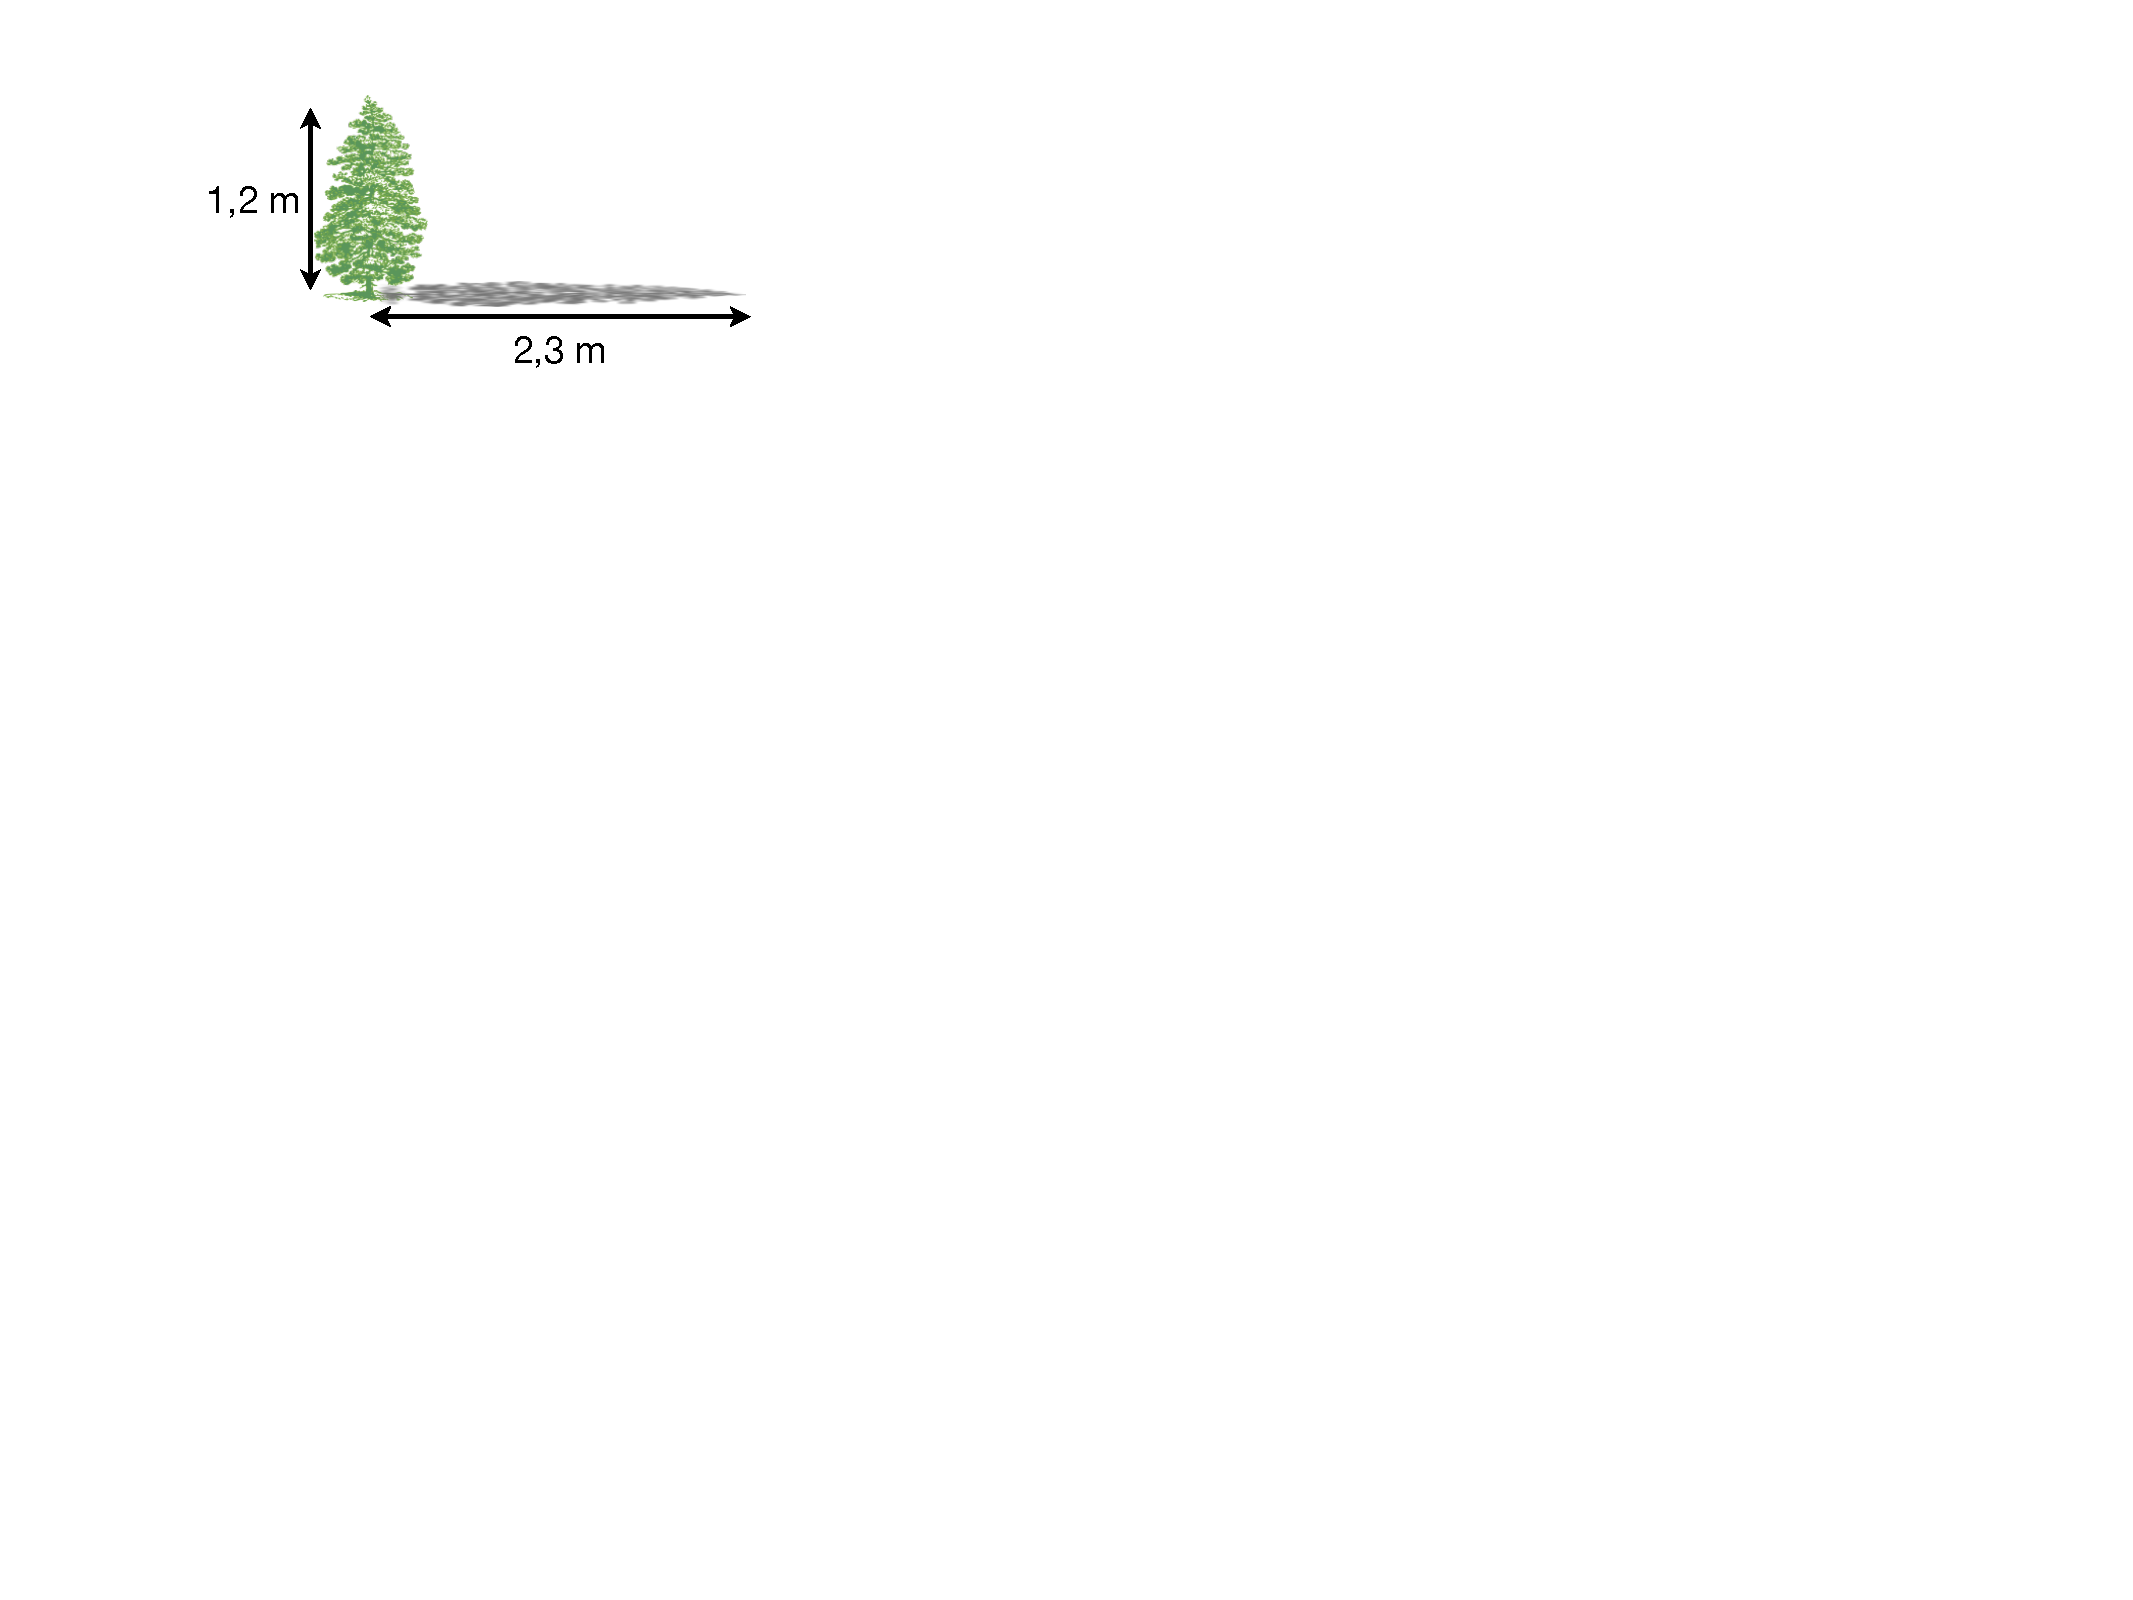
\includegraphics[width=0.9\textwidth]{img-07/arbre}
\end{minipage}

 \answers{Altura arbre $h=\frac{4.2 \cdot 1.2}{2.3}=2.1$ m.}
 

\exer
  Un llibre de 420 pàgines pesa 200 g. Quant pesarà un llibre de la
  mateixa col·lecció de 300 pàgines?
\exer \spen
  Completa la taula de proporció directa.
  Calcula la raó de proporcionalitat.
 
\begin{center}
\begin{tabular}[]{@{}p{1cm}|p{1cm}|p{1cm}|p{1cm}|p{1cm}|p{1cm}|p{1cm}@{}}
\toprule
Litres & 16 & 4,5 & & 1 & & 50\tabularnewline
\midrule
Euros & 36 & & 8,10 & & 10 &\tabularnewline
\bottomrule
\end{tabular}
\end{center}

\answers{
	\begin{tabular}{|c|c|c|c|c|c|c|}
		\hline
		Litres & 16 & 4,5 & 3,6& 1 & 4,44 & 50\tabularnewline\hline
		Euros & 36 &10,125 & 8,10 &2,5 & 10 & 112,5\tabularnewline\hline
	\end{tabular}
	\par
	La raó és $r=\frac{16}{36}=\frac{4}{9}=0.44\cdots$
}


\exer
  Hem gastat 72 l de benzina per recórrer 960 km. Quants litres
  necessitarem per a una distància de 1500 km?
  
  \answers{$\frac{1500\cdot 72}{960}=112,5$ litres}
  
  
\exer
  El meu cotxe gasta 6 litres de benzina cada 100 km, quants litres
  gastarà en un viatge de 1250 km?

\answers{$\frac{1250\cdot 6}{100}=75$ litres}

\exer
  Sis persones realitzen un viatge de vuit dies i paguen en total 40800
  \euro{}. Quant pagaran 15 persones si el seu viatge dura 5 dies?

\answers{És compost, però ho reduïm a simples\par
$\frac{\frac{40800}{6} \cdot 5}{8} 15 = 63750 \euro{}$}

\exer
  La distància real entre dos pobles és 18,5 km. Si en el mapa estan a
  10 cm de distància. A quina escala està dibuixat?

\answers{A escala $1:185\,000$}

\exer
  Quina altura té un edifici si la seva maqueta construïda a escala 1 :
  300 presenta una altura de 12 cm?

\answers{$h =300\times 12=3600$ cm $= 36$ m}


\exer
  Dibuixa l'escala gràfica corresponent a l'escala 1:60000.

\answers{Solució:\par 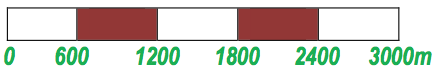
\includegraphics[width=3.4cm]{img-sol/t7-11}}

\exer
  Les dimensions d'una superfície rectangular en el plànol són 6 cm i 14
  cm. Si està dibuixat a escala 1 : 40, calcula les seves mesures reals.


\answers{$6\times 40 =   240$ cm;  $14\times  40=   560$ cm}

\end{mylist}

\begin{theorybox}
  Dues magnituds A i B estan relacionades amb una regla de
  \textbf{proporcionalitat inversa} si:

  - Quan es \textbf{multiplica A} per un factor, \textbf{B resulta
  dividit} pel mateix factor o

  - Quan es \textbf{divideix A} per un factor, \textbf{B resulta
  multiplicat} pel mateix factor.
\end{theorybox}

\begin{mylist}
\exer \spen
 Calcula la raó de
  proporcionalitat i completa la taula de proporcionalitat inversa:

\begin{center}
\begin{tabular}[]{@{}p{2.5cm}|p{1cm}|p{1cm}|p{1cm}|p{1cm}|p{1cm}|p{1cm}@{}}
\toprule
Magnitud A & 36 & 0,09 & & 12 &\tabularnewline
\midrule
Magnitud B & 0,25 & & 6 & & 72\tabularnewline
\bottomrule
\end{tabular}
\end{center}

\answers{\begin{tabular}{|c|c|c|c|c|c|c|}\hline
	 	Magnitud A & 36 & 0,09 & 1,5& 12 & 0,125\tabularnewline\hline
		 Magnitud B & 0,25 & 100 & 6 & 0,75 & 72\tabularnewline\hline
\end{tabular}\par
Raó $r'=36\cdot 0.25 = 9$
}


\exer
  En tallar una quantitat de fusta hem aconseguit 6 panells de 2,25 m de
  llarg. Quants panells aconseguirem si ara fan 1,5 m de llarg?
  
  \answers{$\frac{2,25\times 6}{1,5}=9$ panells de fusta}
  
  
\exer
  Per omplir un dipòsit s'obren tres aixetes que donen 2 litres per
  minut cadascuna i triguen 6 hores. Quant temps trigaran 4 aixetes
  similars que donen 5 litres per minut cadascun?

\answers{$\frac{3\times 2 \times 6}{4 \times 5}=1,8$ hores. És a dir, tardarà 1 hora i 48 minuts.}

\begin{comment}
\exer
Tres màquines fabriquen 1200 peces funcionant 5 hores diàries. Quantes
màquines s'han de posar a funcionar per aconseguir 6000 peces durant 9
hores diàries?
\end{comment}

\exer
  En la construcció d'un pont de 900 m s'han utilitzat 250 bigues, però
  l'enginyer no està  segur i decideix reforçar l'obra afegint 75
  bigues més. Si les bigues es col·loquen uniformement al llarg de tot
  el pont, a quina distància es col·locaran?

\answers{$\frac{900}{75}=12$ m.}

\begin{comment}
\exer
  Aquest mateix hort necessita 1200 caixes per envasar les seves
  mandarines en caixes d'un quilogram. Quantes caixes necessitaria per
  envasar-les en caixes de mig quilogram? I per envasar-les en caixes de
  2 quilograms?
\end{comment}

\end{mylist}


\section{Proporcionalitat composta}


\begin{mylist}
	\exer El lloguer de 2 cotxes durant 9
dies costa 675 \euro{}. Quant costarà llogar 5 cotxes durant 7 dies?
\end{mylist}
	\vspace{-0.25cm}
	
\begin{example}
	\begin{minipage}{0.6\textwidth}
		Plantejam el problema amb les tres magnituds que apareixen ``cotxes", ``Dies'' i ``Preu". 
		Ara ens fixam quina és la relació entre la magnitud que ens demanen ``Preu" amb cadascuna de les altres.
		Com més cotxes, major el preu (Directa). Com més dies lloguem, major el preu (Directa).
		
	\end{minipage}
	\begin{minipage}{0.4\textwidth}
		\centering
		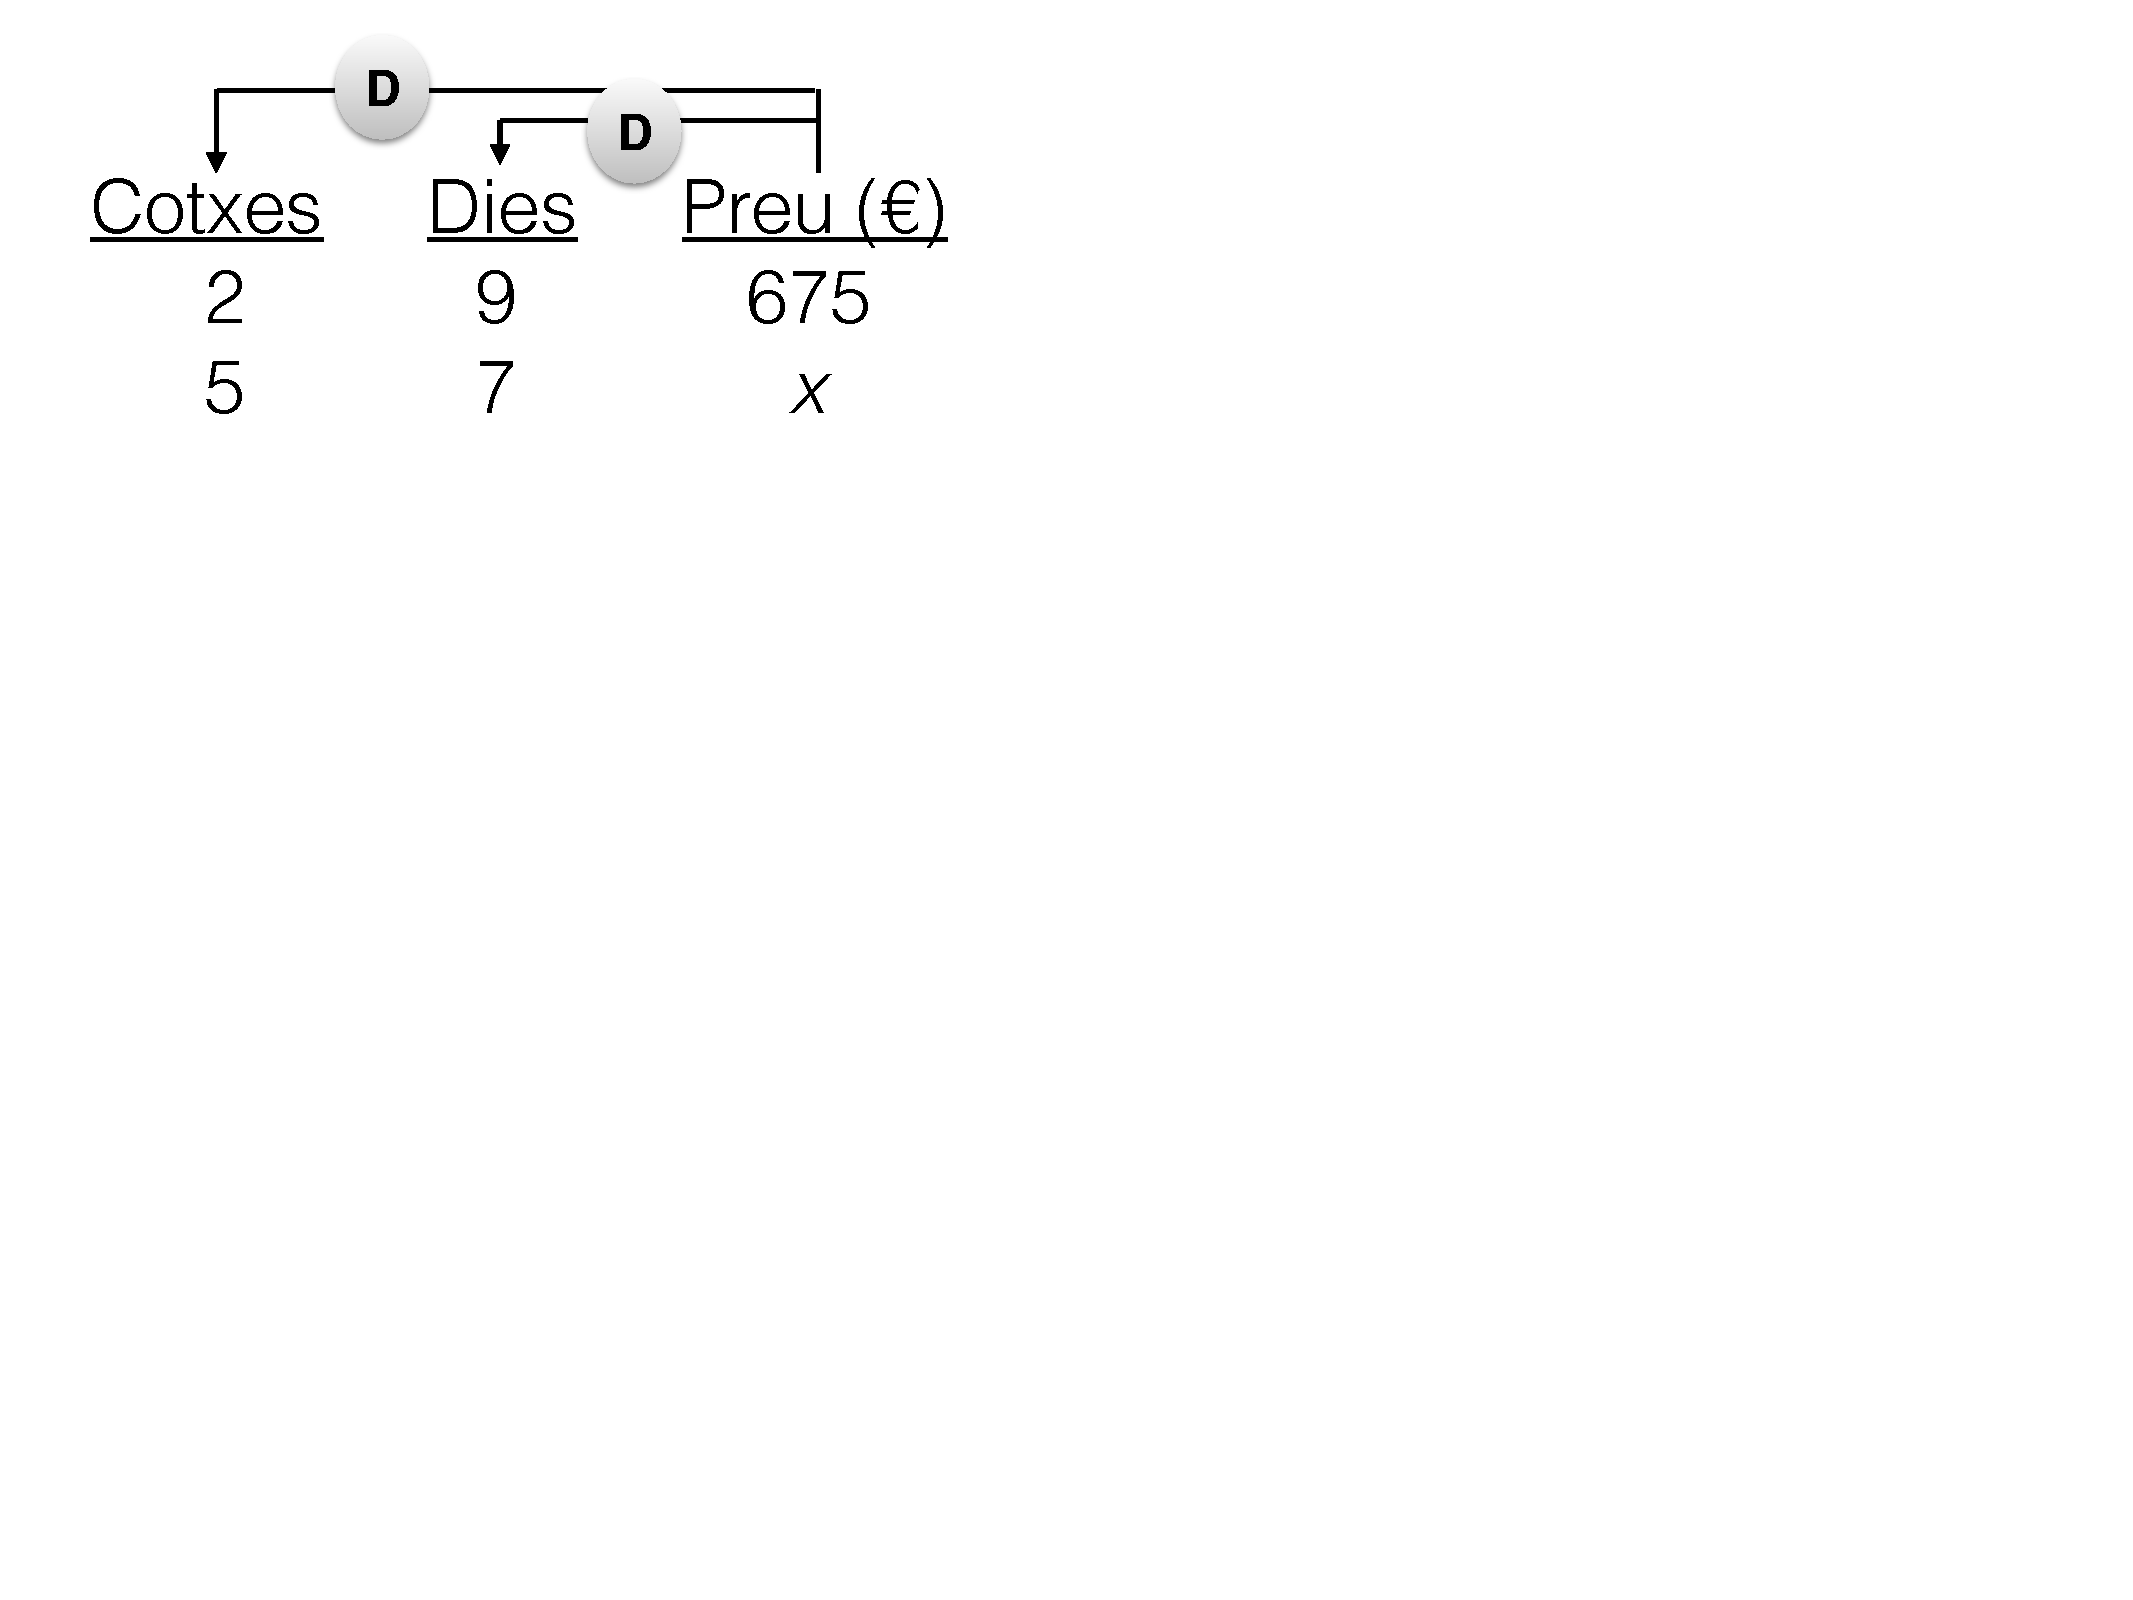
\includegraphics[width=5cm]{img-07/proporcionalitat}
	\end{minipage}
	
	\[ \frac{675}{x} = \frac{2}{5} \cdot \frac{9}{7} = \frac{18}{35} \quad \rightarrow \quad \text{Aïllam la }x \quad x=\frac{675\cdot 35}{18}= 1312,50 \text{ \euro}  \]
\end{example}
 
 
 \begin{mylist}
 
 \exer
 Una barra de metall de 10 m de llarg i 2 cm\textsuperscript{2} de
 secció pesa 8,45 kg. Quant pesarà una barra del mateix material de 5 m
 de llarg i 7 cm\textsuperscript{2} de secció.
 
 \answers{D-D $\frac{10}{5} \cdot  \frac{2}{7} =  \frac{8.45}{x}$ $\, \rightarrow \, x=14.79$ kg}
 
 \exer
 Sabem que dues màquines funcionant 6 hores diàries consumeixen 1500
 kW/h al dia. Durant quantes hores al dia haurien de treballar 5
 màquines si volem que el consum no superi els 5000 kW/h?
 
 \answers{I-D $\frac{5}{2} \cdot  \frac{1500}{5000} =  \frac{6}{x}$ $\, \rightarrow \, x=8$ hores}
 
 \exer
 Si 12 excavadores fent feina 10 dies han remogut 360
 m\textsuperscript{3} de terra, quants de dies tardaran 8 excavadores a
 remoure 620 m\textsuperscript{3} de terra?
 
 \answers{I-D $\frac{8}{12} \cdot  \frac{360}{620} =  \frac{10}{x}$ $\, \rightarrow \, x=25.83$ dies}
  
\exer Tres treballadors recullen 300 kg de raïm en 2 dies. Quant tardaran 4 treballadors a recollir 500 kg del mateix raïm?
 

\end{mylist}

\begin{example}
	
	\begin{minipage}{0.6\textwidth}
		Plantejam el problema amb les tres magnituds que apareixen ``Treballadors", ``Kg raïm'' i ``Dies". 
		Ara ens fixam quina és la relació entre la magnitud que ens demanen ``Dies" amb cadascuna de les altres.
		Com més treballadors, menys dies (Inversa). Com més Kg, més dies (Directa).
		
	\end{minipage}
	\begin{minipage}{0.4\textwidth}
		\centering
		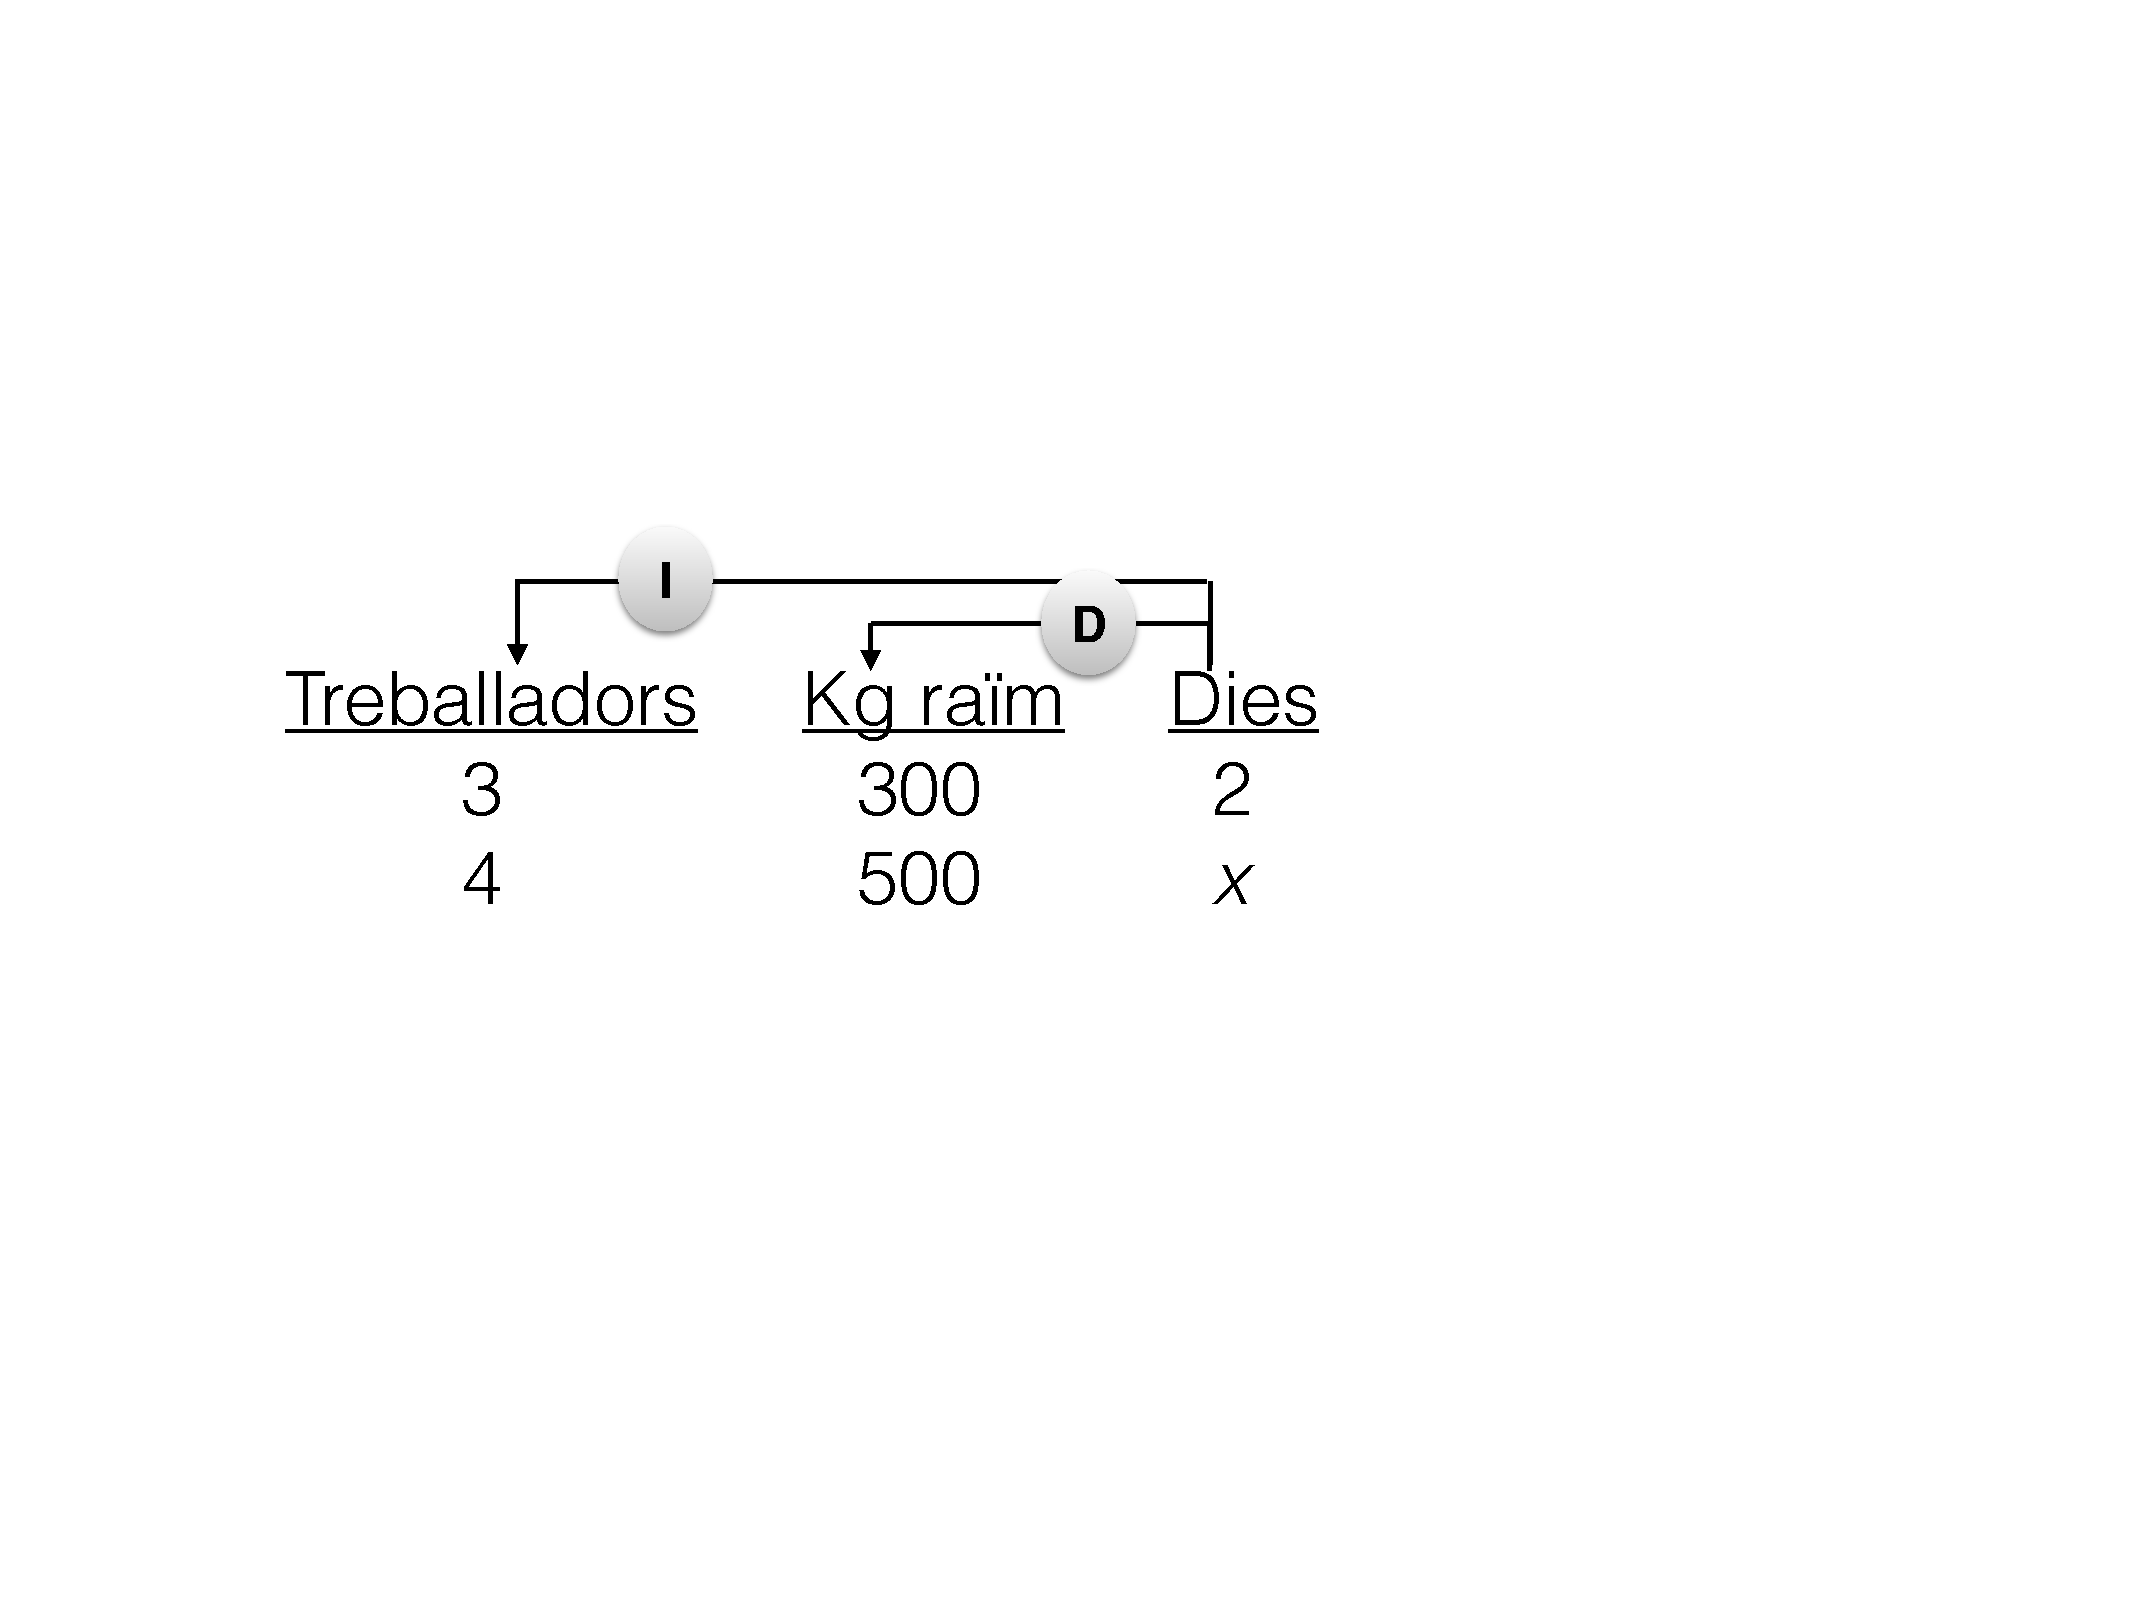
\includegraphics[width=5cm]{img-07/proporcionalitat2}
	\end{minipage}
	
	\[ \frac{2}{x} = \boxed{ \frac{4}{3} } \cdot \frac{300}{500} \quad \rightarrow \quad \text{Aïllam la }x \quad x=\frac{2\cdot 3 \cdot 500}{4\cdot 300}= 2,5 \text{ dies}  \]
	
\end{example}
 
 
 \begin{mylist}
 	

\exer
  Un total de 18 operaris, fent feina 6 hores diàries, han tardat 6 dies
  a instal·lat 300 m de cable. Quantes hores diàries han de fer feina 24
  operaris durant 14 dies per instal·lar 700 m de cable?

 \answers{I-I-D $\frac{24}{18} \cdot  \frac{14}{6} \cdot  \frac{300}{700}=  \frac{6}{x}$ $\, \rightarrow \, x=4.5$ hores diàries}

\exer
  L'any passat teníem un pressupost per al menjador de l'escola de
  34.000 \euro{} mensuals per alimentar 262 alumnes. Si aquest any hi ha
  22 alumnes més però el pressupost només ha augmentat en 1.200 \euro{}
  mensuals, serà possible oferir el servei de menjador? (\textit{Suposa un mes de 30 dies})
 \answers{D-I $\frac{34000}{35200} \cdot  \frac{262}{284} =  \frac{k}{x}$ $\, \rightarrow \, x=0.9551\, k$; si entenem $k=30$ dies $x=28.65$; si $k=31$ dies $x=29.6$; i si $k=365$ dies $x=348.61$ dies}

\exer
  Sabem que 9 ordinadors encesos durant 10 hores diàries produeixen una
  despesa de 2340 \euro{} anuals. Quina seria la despesa si
  s'encenguessin 6 ordinadors més durant una hora menys al dia?

 \answers{D-D $\frac{9}{15} \cdot  \frac{10}{9} =  \frac{2340}{x}$ $\, \rightarrow \, x=3510$ \euro{}/anuals}

\exer
  Una família de sis membres consumeix 2 kg de pa cada 5 dies. Quants de
  dies els durarien 3 kg de pa a una família de 8 membres amb un consum
  similar?

 \answers{I-D $\frac{8}{6} \cdot  \frac{2}{3} =  \frac{5}{x}$ $\, \rightarrow \, x=5.6$ dies}

\exer
  Amb quatre fotocopiadores es fan 30.000 còpies fent feina 3 hores
  diàries. Quantes còpies es podrien fer amb 5 fotocopiadores fent feina
  durant 2 hores diàries?

 \answers{D-D $\frac{4}{5} \cdot  \frac{3}{2} =  \frac{30000}{x}$ $\, \rightarrow \, x=25\,000$ còpies.}

\end{mylist}


\section{Repartiments proporcionals}

\begin{mylist}
	\exer
	Cinc persones comparteixen loteria, amb 10, 6, 12, 7 i 5
	participacions respectivament. Si han obtingut un premi de
	18000~\euro{}, quant correspon a cadascun?
	
	\answers{Directa: $10 + 6+ 12+ 7 + 5=40$; $\frac{10}{40} 18000=4500$, $\frac{6}{40} 18000=2700$, $\frac{12}{40} 18000=5400$, $\frac{7}{40} 18000=3150$, $\frac{5}{40} 18000=2250$ \euro{}}
	
	\exer
	En el testament, l'avi estableix que vol repartir entre els seus néts
	22200 \euro{}, de manera proporcional a les seves edats, 12, 15 i 18
	anys, mirant que la major quantitat sigui per als néts majors. Quant
	rebrà cadascun?
	
	\answers{Directa: $12+15+18=45$. Rebran $\frac{12}{45}\,22200=5920$,  $\frac{15}{45}\,22200=7400$,
	$\frac{18}{45}\,22200=8880$ \euro{}}
	
	\exer
	Tres pagesos s'encarreguen del cultiu de la vinya. El primer va treballar 32 hores, el segon 24 i el tercer 14. Els beneficis són de 7350 \euro{}. Quant li toca a cadascun?
	
	\answers{$32+24+14=70$; Rebran: $\frac{32}{70}\, 7350=3360$, $\frac{24}{70}\, 7350=2520$ i $\frac{14}{70}\, 7350=1470$ \euro{} }
\end{mylist}

\pagebreak

\begin{resolt}{
Un avi decideix repartir 6.000 € entre els seus tres néts, però en comptes de donar-los un terç a cadascun prefereix fer-ho de forma proporcional a l'edat de cada nét, que tenen 7, 12 i 21 anys. Quant rebrà cadascun d'ells?
	}
	El total d'anys és 7+12+21 = 40. El repartiment proporcional directe per cada nét és:
	
	Pel de 7 anys: $\frac{7}{40} \,\, de\,\,  6000 =1050$ \euro. 
	
	Pel de 12 anys: $\frac{12}{40} \,\, de \,\, 6000 =1800$ \euro. 
	
	Pel de 21 anys: $\frac{21}{40} \,\, de\,\,  6000 =3150$ \euro. 
\end{resolt}

\begin{mylist}


\exer
  En el testament, l'avi estableix que vol repartir entre els seus néts
  22200 \euro{}, de manera proporcional a les seves edats, 12, 15 i 18
  anys, cuidant que la major quantitat sigui per als néts menors. Quant
  rebrà cadascun?
  
  		\answers{Inversa: $\frac{1}{12}+\frac{1}{15}+\frac{1}{18}=\frac{15}{180}+\frac{12}{180}+\frac{10}{180}=\frac{37}{180}$. Cadascun rebrà: $\frac{15}{37}\, 22200=9000$, $\frac{12}{37}\, 22200=7200$, $\frac{10}{37}\, 22200=6000$ \euro{}}
  	
\exer
  Tres socis han invertit 20000 \euro{}, 34000 \euro{} i 51000 \euro{}
  aquest any en la seva empresa. Si els beneficis a repartir a final
  d'any ascendeixen a 31500 \euro{}, quant correspon a cadascun?

	\answers{$\frac{20000}{105000} \,31500=6000$, $\frac{34000}{105000} \,31500=10200$, $\frac{51000}{105000} \,31500=15300$ \euro{}}

\exer
  Calcula el preu del quilo de barreja de dos tipus de cafè: 3,5 kg a
  4,8 \euro{}/kg i 5,20 kg a \linebreak 6 \euro{}/kg.

	\answers{$\frac{3.5\cdot 4.8 + 5.2 \cdot 6}{3.5+5.2}=5.52$ \euro{} }
	
\exer
  Quants litres de suc d'aranja de 2,40 \euro{}/l han de barrejar-se amb
  4 litres de suc de taronja a 1,80 \euro{}/l per obtenir una barreja a
  2,13 \euro{}/l?
  
  	\answers{$\frac{x\cdot 2.4 + 1.8 \cdot 4}{x+4}=2.13 \quad \rightarrow \quad x=\frac{1.32}{0.27}=4.89$ litres. }
  	
  \exer
  En un concurs s'acumula puntuació de forma inversament proporcional al
  nombre d'errors. Els quatre finalistes, amb 6, 5, 2, i 1 error, han de
  repartir-se els 1400 punts. Quants punts rebrà cadascun?
  
  	\answers{Inversa: $\frac{1}{6}+\frac{1}{5}+\frac{1}{2}+\frac{1}{1}=\frac{5}{30}+\frac{6}{30}+\frac{15}{30}+\frac{30}{30}=\frac{56}{30}$. Cadascú rebrà: $\frac{5}{56} \, 1400=125$, $\frac{6}{56} \, 1400=150$, $\frac{15}{56} \, 1400=375$, $\frac{30}{56} \, 1400=750$ punts}
  
  \begin{comment}
\exer
  Calcula la llei d'una joia sabent que pesa 110 g i conté 82 g d'or
  pur. \emph{Nota: La \textbf{llei} d'un \textbf{aliatge} és la relació
  entre el pes del metall més valuós i el pes total.}
\exer
  Quants quirats, aproximadament té la joia anterior? \emph{Cerca a
  internet la conversió entre quirats i mg.}
\end{comment}
\end{mylist}

 
\section{Percentatges}

%  \emph{FONT: Proves d'accés a cicles de grau mitjà} 
\begin{theorybox}
	Si tenim una quantitat total, una part i un percentatge $p$, aquests tres estan relacionat per:
	
	\textbf{Percentatge:}  $ p = \frac{Part}{Total} \cdot 100$ \%
	\quad
	\textbf{Part:}  $ Part = \frac{p}{100} \cdot Total$
	\quad
	\textbf{Total:} $ Total = \frac{100}{p} \cdot Part$
	
	Si ens fan un \textbf{rebaixa} del r \% damunt una quantitat, el preu final és
	$ Final = \frac{100-r}{100} \cdot Inicial $
	
	Si ens fan una \textbf{pujada} del r \% damunt una quantitat, el preu final és
	$ Final = \frac{100+r}{100} \cdot Inicial$
	 
	Al número $i=\frac{100\pm r}{100}$ s'anomena \textbf{índex de variació}.
\end{theorybox}


\begin{mylist}
\exer
  Una finca consta de dos pisos i un local. El tant per cent de
  propietat és del 30 \%, 30 \% i del 40\% respectivament. a) Quina
  fracció de propietat correspon a cada un? b) Les despeses comuns del
  trimestre passat són de 448 euros. Quant li correspon pagar a cada un?
  \answers{[$\frac{3}{10}$; $\frac{3}{10}$, $\frac{4}{10}$, 
  			$134.4$; $134.4$, $179.2$ \euro{}]}
  		
\exer
  Els preus dels articles indicats a una pàgina d'internet no tenen el
  IVA inclòs. Volem comprar 4 bosses de te a 4,25 \euro{} cadascuna i 6
  bosses de cacau a 3,50 \euro{} cadascuna. Si l'IVA que s'aplica a
  aquests productes és del 15\% , Quant haurem de pagar en total?
  
  \answers{$4\cdot 4.25+ 6\cdot 3.50 = 38$; $38\cdot 1.15=43.7$ \euro{}}
  
\exer
  L'any passat un club tenia 250 membres i cada membre va pagar 100
  \euro{} de quota anual. Aquest any el nombre de socis ha augmentat un
  4\% respecte a l'any passat i la quota anual ha augmentat un 10\%
  també respecte a l'any passat. Quants diners ingressarà aquest any el
  club en concepte de quotes de socis?
  
    \answers{$1.04\cdot 250=260$ socis; $1.10\cdot 100 = 110$ \euro{} de quota anual; Ingressarà en total $260 \cdot 110 = 28600$ \euro{}}
  
\exer
  Un medicament val, sense IVA, 14 \euro{}. Amb una recepta mèdica hem
  de pagar el 40\% del preu total. Si sabem que l'IVA és del 4 \%, quant
  haurem de pagar si duim la recepta?
  
    \answers{$1.04 \cdot 0.40 \cdot 14= 5.82$ \euro{}}
    
\exer
  Ricard compra a la peixateria tres quarts de quilo de calamars a 8,60
  \euro{} / Kg i un lluç de 650 grams a 5,80 \euro{} / Kg.

  a ) Quants diners li tornaran si paga amb un bitllet de 20 \euro{} ?

  b ) Si s'ha gastat el 20 \% dels diners que duia, amb quants diners
  ha sortit de casa ?
  
    \answers{[$0.75\cdot 8.60 + 0.650\cdot 5.80 = 10.22$ li ha costat; li tornaran $9.78$ \euro{},  
    	Tenia $0.2\,x = 10.22 \quad \rightarrow \quad x=51.10$ \euro{}]}
    
\exer
  a) Quan a un porc, un cop sacrificat, li treuen les vísceres i els
  budells, queda la canal que pesa un 78 \% del que pesava el porc viu.
  La sobrassada que s'obté de aquest animal correspon a un 52\% del pes
  de la canal. Quants quilos de sobrassada s'obtenen d'un porc que, viu,
  pesava 148 kg?

  b ) Per fer sobrassada es posen 21 grams de sal i 45 grams de pebre
  vermell per cada quilo de pasta. Quants quilos de sal i de pebre
  vermell es necessiten per fer la sobrassada que s'obté del porc de 148
  kg?
  
    \answers{[$0.78 \cdot 0.52 \cdot 148 = 60$ kg de sobrassada,
    		$0.021\cdot 60=1.26$ kg de sal; i $0.045\cdot 60=2.7$ kg de pebre vermell]}
  
\exer
  En un centre hi ha tres grups de 3r d'ESO. S'ajunten per fer una coral
  els que tenen facilitat per entonar. A 3r A hi ha 30 alumnes, en 3r B
  hi ha 28, i en 3r C hi ha 32. Hi participen a la coral el 40 \% dels
  alumnes de 3r A, el 25 \% dels de 3r B, i el 75\% dels de 3r C. a)
  Quants alumnes formen la coral? b ) Els que formen el coral, quin
  percentatge del total d'alumnes de 3r d'ESO representen?
  
    \answers{[$0.4\cdot 30 + 0.25\cdot 28 + 0.75 \cdot 32 = 43$ alumnes participen a la coral,
    El total d'alumnes és $30+28+32=90$; $\frac{43}{90}\cdot 100=47.78$ \% del total]}
    
\exer
  L'aire és una mescla de gasos. En l'atmosfera la seva composició és
  aproximadament: el 78\% de nitrogen, 21\% d'oxigen, 0,04\% de diòxid
  de carboni i la resta són gasos nobles.

  a) Quin és el percentatge de gasos nobles que hi ha a l'aire?

  b) Comptant que una persona adulta normal inspira 500 ml d'aire cada
  vegada que respira, i suposant que respira 15 vegades per minut,
  calcula quants litres de cadascun dels gasos esmentats s'inspira en
  una hora.
  
   \answers{[$100-78-21-0.04=0.96$ \% de gasos nobles,
   			$\frac{0.96}{100}\,500 \cdot 15 \cdot 60 = 4320$ ml/hora = 4.32 l/hora]}
    
\exer
  a) Una persona compra un equip de música que val a 500 \euro{}. Li fan
  un 20\% de descompte però ha de pagar un 16 \% d'IVA. Quant li costarà?

  b) Si paga al comptat un 25 \% del preu i la resta en un any sense
  interessos, quant haurà de pagar cada mes?
  
    \answers{[$0.8\cdot 1.16\cdot 500=464$ \euro{}, $\frac{0.75\cdot 464}{12}=29$ \euro{}/mensuals]}

  \begin{comment}
\exer
  a) Una persona compra una finca per 32.000 \euro{}. La gestoria , per
  fer els tràmits, li cobra l'equivalent a un 1,5 \% d'aquesta quantitat
  ; i el notari, un 1,2 \%. Quant ha de pagar en total?

  b ) D'aquesta quantitat paga un 75\% al comptat i la resta, al cap
  d'un any, amb un recàrrec del 4 \%. Quant pagarà per aquest segon
  rebut?

\exer
  Una botiga de roba fa la següent publicitat: Si compra per valor
  superior a 160 \euro{} li descomptem un 25\% i si el valor de la
  compra és entre 100 i 160 \euro{}, li descomptem un 15 \%. Per a
  imports inferiors no hi ha descompte. Vull comprar-me una tovallola de
  bany i uns vestits de bany. Estic dubtant entre una tovallola blava
  que costa 75 \euro{} i una altra de dos colors que val 95 \euro{}. Els
  banyadors que jo vull valen 71 \euro{}. Quant em costaria en cada cas?
\end{comment}
\end{mylist}

\pagebreak

\section{Interès bancari}

\begin{theorybox}
	Si $C_i$ és el \textbf{capital} inicial que deixam al banc durant $t$ anys a un \textbf{rèdit} $r$ (\%), el capital final s'obté de sumar-li els \textbf{interesos} $C_f = C_i + I$.
	
	Si \textbf{l'interès és simple}, els interesos s'obtenen de la fórmula $I = \frac{r}{100}  \cdot C_i \cdot t $.
	
	Si \textbf{l'interès és compost}, el capital final és directament $C_f=C_i \left( 1 + \frac{r}{100}\right)^t$
\end{theorybox}

\begin{mylist}

\exer
  Calcula l'interès simple que produeixen 105000 \euro{} al 4,8 \%
  durant 750 dies.
  
  \answers{$\frac{105000\cdot 4.8 \cdot 750}{36000}=10500$ \euro{}}
  
\exer
  Al 5 \% d'interès compost durant 12 anys, quin serà el capital final
  que obtindrem en dipositar 39500 \euro{}? Ajuda: també pots utilitzar
  el full de càlcul.
  
    \answers{$39500 \left(1+\frac{5}{100}\right)^{12} = 70936.32$  \euro{}}
    
\exer
  Quin capital cal dipositar a l'1,80 \% durant 6 anys per obtenir un
  interès simple de 777,6 \euro{}?

  \answers{$\frac{C \cdot 1.8 \cdot 6}{100}=777.6$; $C=7200$ \euro{}}
\end{mylist}

%%%%%%%%%%%%%%%%%%%%%%%%%%%%%%%%%%%%%%%%%%%%%%%

\begin{activitats}

\begin{mylist}
\exer
  Copia en el teu quadern, calcula la raó de proporcionalitat i completa
  la taula de proporcionalitat directa:

\begin{tabular}[]{@{}llllll@{}}
\toprule
\textbf{litres} & 6,25 & & 0,75 & 1,4 &\tabularnewline
\midrule
\textbf{euros} & & 15 & 2,25 & & 4,5\tabularnewline
\bottomrule
\end{tabular}

\answers{\begin{tabular}{|c|c|c|c|c|c|}
		\hline
		\textbf{l.} & 6,25 & 5 & 0,75 & 1,4 &\tabularnewline
			\hline
		\textbf{\euro{}} & 18,75 & 15 & 2,25 &4,2 & 4,5\tabularnewline
			\hline
\end{tabular}\par 
$k=\frac{0.75}{2.25}=\frac{1}{3}$
}


\exer
  Amb 76 \euro{} hem pagat 12,5 m de tela, quant ens costaran 22,5 m?
\answers{136.8 \euro{}}

\exer
  Cada setmana paguem 82 \euro{} en transport. Quant gastarem els mesos
  de juny i juliol?
\answers{Suposant 4 setmanes per mes: $82\cdot 8 =656$ \euro{}. Suposant 9 setmanes en total, $82\cdot 9 =738$ \euro{}. Més precís (per dies): $\frac{82\cdot 61}{7}=714.57$ \euro{} }

\exer
  Per tapissar cinc cadires he utilitzat 2,3 m de tela, quantes
  cadires podré entapissar amb la peça completa de 23 m?
\answers{50 cadires}


\exer
  Un camió ha transportat en 3 viatges 220 sacs de patates de 24 kg
  cadascun. Quants viatges seran necessaris per transportar 550 sacs de
  30 kg cadascun?
  \answers{9,3 = 10 viatges}
  
  
\exer
  Una edició de 350 llibres de 210 pàgines cadascun aconsegueix un pes
  total de 70 kg. Quants kg pesarà una altra edició de 630 llibres de
  140 pàgines cadascun?
  \answers{84 kg}
  
  
\exer
  Sabent que la raó de proporcionalitat directa és $\frac{A}{B}
  = 1,8$, copia en el teu quadern i completa la següent taula:


\begin{tabular}[]{@{}llllll@{}}
\toprule
\textbf{Magnitud A} & 12,6 & & & 4,14 &\tabularnewline
\midrule
\textbf{Magnitud B} & & 9 & 0,1 & & 2,7\tabularnewline
\bottomrule
\end{tabular}

\answers{\begin{tabular}{|c|c|c|c|c|c|}
		\toprule
		\textbf{A} & 12,6 &  16,2 & 0,18 & 4,14 & 4,86\tabularnewline
		\midrule
		\textbf{B} & 7 & 9 & 0,1 & 2,3 & 2,7\tabularnewline
		\bottomrule
\end{tabular}}




\exer
  El model de telèfon mòbil que costava 285 \euro{} + IVA està ara amb
  un 15 \% de descompte. Quin és el seu preu rebaixat? (IVA 21 \%)
  \answers{293,12 \euro{}}
  
  
\exer
  Per retardar-se dos mesos en el pagament d'un deute de 1520 \euro{},
  una persona ha de pagar un recàrrec del 12\%, quant ha de retornar en
  total?
  \answers{1702,40 \euro{}}
  
  
\exer
  Quin tant per cent de descompte s'ha aplicat en una factura de 1820
  \euro{} si finalment es van pagar 1274 \euro{}?
  \answers{30 \%}
  
  
\exer
  En comprar un televisor he obtingut un 22 \% de descompte, per la qual
  cosa al final he pagat 483,60 \euro{}, quin era el preu del televisor
  sense descompte?
  \answers{620 \euro{}}
  
  
 \pagebreak
  
\exer
  Per liquidar un deute de 3500 \euro{} abans del previst, una persona
  paga finalment 3080 \euro{}, quin percentatge del seu deute s'ha
  estalviat?
  \answers{S'han estalviat 420 \euro{}; El percentatge és 12 \%}
  
  
\exer
  El preu d'un viatge s'anuncia a 907,50 \euro{} IVA inclòs. Quin era el
  preu sense IVA? (IVA 21 \%)
  \answers{El preu sense IVA és 750 \euro{}}
  
  
\exer
  Quin increment percentual s'ha efectuat sobre un article que abans
  valia 38 \euro{} i ara es paga a 47,12 \euro{}?
  \answers{24 \%}
  
  
%\exer
%  Un mapa està dibuixat a escala 1:700000. La distància real entre dues
%  ciutats és 21 km. Quin és la seva distància en el mapa?
\exer
  La distància entre Oviedo i La Corunya és de 340 km. Si en el mapa
  estan a 10 cm, quina és l'escala a la qual està dibuixat?
 \answers{1 : 3400000}
 


\exer
 Completa la següent taula:


\begin{tabular}[]{@{}l|l|l@{}}
\toprule
\textbf{Dibuix} & \textbf{Real} &
\textbf{Escala}\tabularnewline  
\midrule
24 cm $\times$ 5 cm & & 1:25000\tabularnewline \hline
6 cm & 15 km &\tabularnewline \hline
& 450 m & 1:30000\tabularnewline 
\bottomrule
\end{tabular}
\answers{6 km llarg i 1.25 km d'ample; 1:250000; 1.5 cm}




\exer
  Copia en el teu quadern, calcula la raó de proporcionalitat inversa i
  completa la taula:

\begin{tabular}[]{@{}l|l|l|l|l|l@{}}
\toprule
\textbf{Magnitud A} & 4 & 7,5 & & 3,6 &\tabularnewline
\midrule
\textbf{Magnitud B} & & 12 & 0,18 & & 10\tabularnewline
\bottomrule
\end{tabular}

\answers{\begin{tabular}{|c|c|c|c|c|c|}
		\hline
		\textbf{ A} & 4 & 7,5 & 500 & 3,6 & 9\tabularnewline
		\hline
		\textbf{ B} & 22.5 & 12 & 0,18 & 25& 10\tabularnewline
		\hline
\end{tabular}\par 
$k'=7.5\times 12 = 90$}




\exer
  Quina velocitat ha de portar un automòbil per recórrer en 4 hores
  certa distància si a 80 km/h ha trigat 5 hores i 15 minuts?
  
  \answers{Espai recorregut 420 km. Velocitat 105 km/h}
  
  
  
  \begin{comment}
  \exer
  La raó de proporcionalitat inversa entre A i B és 5,4. Copia en el teu
  quadern i completa la taula següent:


\begin{tabular}[]{@{}l|l|l|l|l|l@{}}
\toprule
\textbf{A} & 18 & & 9 & & 10,8\tabularnewline
\midrule
\textbf{B} & & 0,03 & & 2,7 &\tabularnewline
\bottomrule
\end{tabular}

\end{comment}



\exer
  En la granja es fa la comanda de farratge per alimentar a 240 vaques
  durant 9 setmanes. Si ven 60 vaques, quantes setmanes li durarà el
  farratge? I si en lloc de vendre, compra trenta vaques? I si decideix
  rebaixar la ració una quarta part amb les 240 vaques?
  
  \answers{12 setmanes; 8 setmanes; 12 setmanes}
  
  
\exer
  Amb dotze paquets de 3,5 kg cadascun poden menjar 80 gallines
  diàriament. Si els paquets fossin de 2 kg, quants necessitaríem per
  donar de menjar a les mateixes gallines?
  \answers{42 kg en total; Número de paquets 21.}
  
  
  
  \begin{comment}
\exer
  Determina si les dues magnituds són directa o inversament
  proporcionals i completa la taula en el teu quadern:


\begin{tabular}[]{@{}l|l|l|l|l|l|l@{}}
\toprule
\textbf{A} & 24 & 8 & 0,4 & 6 & & 50\tabularnewline
\midrule
\textbf{B} & 3 & 9 & 180 & & 20 &\tabularnewline
\bottomrule
\end{tabular}
\end{comment}

\exer
  Si la jornada laboral és de 8 hores necessitem a 15 operaris per
  realitzar un treball. Si rebaixem la jornada en mitja hora diària,
  quants operaris seran necessaris per realitzar el mateix treball?
  \answers{16 operaris}
  
  
  
\exer
  En un magatzem es guarden reserves de menjar per 80 persones durant 15
  dies amb 3 racions diàries, quants dies duraria el mateix menjar per a
  75 persones amb 4 racions diàries?

\answers{12 dies}


\exer
  Deu operaris instal·len 3600 m de tanca en 6 dies. Quants dies
  trigaran 12 operaris a instal·lar 5040 m de tanca?

\answers{7 dies}


\exer
  En un concurs el premi de 168000 \euro{} es reparteix de forma
  directament proporcional als punts aconseguits. Els tres finalistes
  van aconseguir 120, 78 i 42 punts. Quants euros rebran cadascun?
\answers{84000 \euro{}; 54600 \euro{}; 29400 \euro{}}



\exer
  Un treball es paga a 3120 \euro{}. Tres operaris ho realitzen aportant
  el primer 22 jornades, el segon 16 jornades i el tercer 14 jornades.
  Quant rebrà cadascun?
\answers{1320 \euro{}; 960 \euro{}; 840 \euro{}}


\exer
  Cinc persones comparteixen un microbús per realitzar diferents
  trajectes. El cost total és de 157,5 \euro{} més 20 \euro{} de
  suplement per servei nocturn. Els quilòmetres recorreguts per cada
  passatger van ser 3, 5, 7, 8 i 12 respectivament. Quant ha d'abonar
  cadascun?
\answers{Suposant un repartiment proporcional de 177.5 \euro{}, cadascú ha de pagar: 15.21 \euro{}; 25.36 \euro{}; 35.5 \euro{}; 40.57 \euro{}; 60.86 \euro{}.}


\exer
  S'ha decidit penalitzar a les empreses que més contaminen. Per a això
  es reparteixen 2350000 \euro{} per subvencionar a tres empreses que
  presenten un 1 \%, 9\% i 15\% de grau de contaminació. Quant rebrà
  cadascuna?
\answers{9791666,7 \euro{};  5875000 \euro{};  7833333.3 \euro{}}


\exer
  Barregem 3 kg d'ametlles a 14 \euro{}/kg, 1,5 kg de nous a 6
  \euro{}/kg, 1,75 kg d'anacards a 18 \euro{}/kg. Calcula el preu final
  del paquet de 250 g de barreja de fruita seca.
\answers{Preu per kg: 13.2 \euro{}; preu del paquet 3.3 \euro{}}

   
\exer
  Calcula el preu del litre de suc que s'aconsegueix barrejant 8 litres
  de suc de pinya a 2,5 \euro{}/l, 15 litres de suc de taronja a 1,6
  \euro{}/l i 5 litres de suc de raïm a 1,2 \euro{}/l. A quant ha de
  vendre's una ampolla de litre i mig si se li aplica un augment del
  40~\% sobre el preu de cost?

\answers{Preu per litre de mescla: 1.79 \euro{}; Preu per botella: 2.69 \euro{}; Amb l'augment 3.75 \euro{}.}

%\exer
%  Per aconseguir un tipus de pintura es barregen tres productes 5 kg del
%  producte X a 18 \euro{}/kg, 19 kg del producte Y a 4,2~\euro{}/kg i 12
%  kg del producte Z a 8 \euro{}/kg. Calcula el preu del kg de barreja.

\pagebreak

\exer
  Quin capital cal dipositar al 3,5 \% de rèdit en 5 anys per obtenir un
  interès simple de 810 \euro{}?

\answers{4628,57 \euro{}}


\exer
  Quin és el capital final que es rebrà per dipositar 25400 \euro{} a
  l'1,4 \% en 10 anys?

\answers{28956 \euro{}}

\exer
  Quants mesos ha de dipositar-se un capital de 74500 \euro{} al 3 \%
  per obtenir un interès de 2980\euro{}?
 
\answers{16 mesos}


\end{mylist}
\end{activitats}



\begin{autoaval}{46}

\begin{mylist}

\exer[2]
  Completen la taula de proporcionalitat directa:

\begin{center}
\begin{tabular}[]{|p{1.2cm}|p{1.2cm}|p{1.2cm}|p{1.2cm}|p{1.2cm}|p{1.2cm}|}
\hline
\cellcolor{lightgray}
\begin{minipage}[b]{0.16\columnwidth}\raggedright\strut

\textbf{A}
\strut
\end{minipage} & \begin{minipage}[b]{0.16\columnwidth}\raggedright\strut

8
\strut
\end{minipage} & \begin{minipage}[b]{0.16\columnwidth}\raggedright\strut

0,75
\strut
\end{minipage} & \begin{minipage}[b]{0.16\columnwidth}\raggedright\strut
\strut
\end{minipage} & \begin{minipage}[b]{0.16\columnwidth}\raggedright\strut

4,5
\strut
\end{minipage} & \begin{minipage}[b]{0.16\columnwidth}\raggedright\strut

100
\strut
\end{minipage}\tabularnewline \hline
\cellcolor{lightgray}
\begin{minipage}[t]{0.16\columnwidth}\raggedright\strut

\textbf{B}
\strut
\end{minipage} & \begin{minipage}[t]{0.16\columnwidth}\raggedright\strut
\strut
\end{minipage} & \begin{minipage}[t]{0.16\columnwidth}\raggedright\strut

15
\strut
\end{minipage} & \begin{minipage}[t]{0.16\columnwidth}\raggedright\strut

6
\strut
\end{minipage} & \begin{minipage}[t]{0.16\columnwidth}\raggedright\strut
\strut
\end{minipage} & \begin{minipage}[t]{0.16\columnwidth}\raggedright\strut
\strut
\end{minipage}\tabularnewline
\hline
\end{tabular}
\end{center}

\begin{comment}
\begin{tasks}(3)
	\task  160; 0,3; 90; 2000 
	\task  16, 3, 90, 200 
	\task  160, 3, 9, 20
\end{tasks}
\end{comment}
\answers{160; 0.3; 90; 2000}



\exer[2]  Amb 450 \euro{} paguem les despeses de gas durant 8 mesos.
Què pagarem en 30 mesos?

\begin{comment}
\begin{tasks}(3)
	\task  1850 \euro{} 
	\task  1875 \euro{} 
	\task  1687,5 \euro{}
\end{tasks}
\end{comment}
\answers{1687.5 \euro{}}


\exer[2]  Un ordinador que costava 1600 \euro{} s'ha rebaixat a 1400
\euro{}. Quin és el percentatge de rebaixa aplicat?

\begin{comment}
\begin{tasks}(4)
	\task  12,5 \% 
	\task  14 \% 
	\task  15,625 \% 
	\task  16,25 \%
\end{tasks}
\end{comment}
\answers{12.5 \%}


\exer[2]  Per envasar 360 litres d'aigua, quantes botelles
necessitarem si volem utilitzar envasos de tres quarts de litre?

\begin{comment}
\begin{tasks}(4)
	\task  440 botelles 
	\task  280 botelles 
	\task  480 botelles 
	\task  360 botelles
\end{tasks}
\end{comment}
\answers{480 botelles}


\exer[2]  Tres agricultors es reparteixen els quilograms de la collita
de forma proporcional a la grandària de les seves parcel·les. La major,
que mesura 15 ha rep 24 tones. Què rebran la segona  i la tercera si tenen una superfície de  10 ha de 8 ha respectivament?

\begin{comment}
\begin{tasks}(4)
	\task  16 t i 5 t 
	\task  12,8 t i 16 t 
	\task  16 t i 12,8 t 
	\task  16 t i 11 t
\end{tasks}
\end{comment}
\answers{16 t i 12.8 t}


\exer[2]  A quina escala s'ha dibuixat un mapa en el qual 3,4 cm
equivalen a 1,02 km?

\begin{comment}
\begin{tasks}(4)
	\task  1:34000 
	\task  1:3000 
	\task  1:30000 
	\task  1:300
\end{tasks}
\end{comment}
\answers{1:30\,000}


\exer[2]  Amb 4 rotllos de paper de 5 m de llarg, puc folrar 32
llibres. Quants rotllos necessitarem per folrar 16 llibres si ara els
rotllos de paper són de 2 m de llarg?

\begin{comment}
\begin{tasks}(4)
	\task  3 rotllos 
	\task  5 rotllos 
	\task  4 rotllos 
	\task  2 rotllos
\end{tasks}
\end{comment}
\answers{5 rotllos}


\exer[2]  
Quin és el preu final de la mescla formada per 5 kg de farina classe A,
a 1,2 \euro{}/kg, 2,8 kg classe B a 0,85 \euro{}/kg i 4 kg classe C a 1
\euro{}/kg?

\begin{comment}
\begin{tasks}(4)
	\task  1,12\euro{} 
	\task  0,98 \euro{} 
	\task  1,03\euro{} 
	\task  1,05\euro{}
\end{tasks}
\end{comment}
\answers{1,05\euro{}}


\exer[2]  Per transportar 40 tones de mercaderies en 8 dies es
necessiten 24 camions. Quants de camions fan falta per transportar el
doble de mercaderies en 6 dies?
 
\begin{comment}
\begin{tasks}(4)
	\task  64 camions 
	\task  42 camions 
	\task  18 camions 
	\task  12 camions
\end{tasks}
\end{comment}
\answers{64 camions}


\exer[2] En quant es converteixen 1400 \euro{} col·locats al 2~\% d'interès simple durant 6 anys?

\begin{comment}
\begin{tasks}(4)
	\task  16225,35 \euro{} 
	\task  16329,35 \euro{} 
	\task  16240,00 \euro{} 
	\task  14550,00 \euro{}
\end{tasks}
\end{comment}
\answers{16329,35 \euro{}}

\end{mylist}
\end{autoaval}



\pagebreak
\mbox{}
\vspace*{-0.4cm}
\resum
 
\begin{longtable}{|p{0.2\textwidth}|p{0.35\textwidth}|p{0.38\textwidth}|} \hline
\cellcolor{lightgray}\begin{minipage}[t]{0.22\columnwidth}\raggedright\strut
\textbf{Proporcionalitat directa}\strut
\end{minipage} & \begin{minipage}[t]{0.35\columnwidth}\raggedright\strut
Dues magnituds són \textbf{directament} \textbf{proporcionals} quan en
multiplicar o dividir a la primera per un nombre, la segona queda
multiplicada o dividida pel mateix nombre.

La \textbf{raó de proporcionalitat directa} \emph{\textbf{k}}: és
el quocient del valors d'una
variable entre l'altra.\strut
\end{minipage} & \begin{minipage}[t]{0.38\columnwidth}\raggedright\strut
Per empaperar 300 m\textsuperscript{2} hem utilitzat 24 rotllos de
paper, si ara la superfície és de 104 m\textsuperscript{2}, necessitarem
8.32 rotllos, \emph{ja que}

 $k = 300/24 = 12.5$  i  $12.5 = 104/x$
 
 
\emph{per tant} $x = 104/12.5 = 8.32$.\strut
\end{minipage}\tabularnewline \hline

	

\cellcolor{lightgray}
\begin{minipage}[t]{0.22\columnwidth}\raggedright\strut
\textbf{Proporcionalitat inversa}\strut
\end{minipage} & \begin{minipage}[t]{0.35\columnwidth}\raggedright\strut
Dues magnituds són \textbf{inversament} \textbf{proporcionals} quan en
multiplicar o dividir a la primera per un nombre, la segona queda
dividida o multiplicada pel mateix nombre.

La \textbf{raó de proporcionalitat inversa} \emph{k´} és el producte de
cada parell de magnituds:

k' = a · b = a'· b'\strut
\end{minipage} & \begin{minipage}[t]{0.38\columnwidth}\raggedright\strut
Dues persones pinten un habitatge en 4 dies treballant 9 h diàries. Per
pintar el mateix habitatge, 3 persones, treballant 8 h diàries
trigaran\ldots{} 3 dies\strut
\end{minipage}\tabularnewline\hline

\cellcolor{lightgray}
\textbf{Percentatges } & Raó amb denominador 100. & El 87 \% de 2400 és
$\frac{87\cdot 2400}{100}= 2088$\tabularnewline\hline

\cellcolor{lightgray}
\textbf{Escales} & L'escala és la proporció entre les mesures del dibuix
i les mesures en la realitat. & A escala 1:50000, 35 cm són 17,5 km en
la realitat.\tabularnewline\hline

	
\cellcolor{lightgray}
\begin{minipage}[t]{0.22\columnwidth}\raggedright\strut	
\textbf{Repartiment proporcional directe}\strut
\end{minipage} & \begin{minipage}[t]{0.32\columnwidth}\raggedright\strut
Rep més quantitat qui més parts té.\strut
\end{minipage} & \begin{minipage}[t]{0.32\columnwidth}\raggedright\strut
Repartir directament a 6,10 i 14, 105000 \euro{}

6 + 10 + 14 = 30;
105000 : 30 = 3500

\quad 6 · 3500 = 21000 \euro{};

\quad 10 ·3500 = 35000 \euro{}

\quad 14 · 3500 = 49000 \euro{}\strut
\end{minipage}\tabularnewline\hline

	
	\cellcolor{lightgray}
	\begin{minipage}[t]{0.22\columnwidth}\raggedright\strut
\textbf{Repartiment proporcional}

\textbf{Invers}\strut
\end{minipage} & \begin{minipage}[t]{0.35\columnwidth}\raggedright\strut
Rep més quantitat qui menys parts té.\strut
\end{minipage} & \begin{minipage}[t]{0.38\columnwidth}\raggedright\strut
Repartir 5670 inversament a 3, 5 i 6; 

$1/3 + 1/5 + 1/6 = 10/30 + 6/30 +5/30$

\quad 5670 : 21 = 270

\quad\quad 270 · 10 = \textbf{2700;} 

\quad\quad 270 · 6 = \textbf{1620} 

\quad\quad 270 · 5 =\textbf{1350}\strut
\end{minipage}\tabularnewline\hline
 

	
	\cellcolor{lightgray}
	\begin{minipage}[t]{0.22\columnwidth}\raggedright\strut
\textbf{Interès simple}\strut
\end{minipage} & \begin{minipage}[t]{0.35\columnwidth}\raggedright\strut

L'interès és el benefici que s'obté en dipositar un capital en una
entitat financera a un determinat tant per cent durant un temps
\strut
\end{minipage} & \begin{minipage}[t]{0.38\columnwidth}\raggedright\strut
C = 3600; r = 4,3 \%; t = 8 anys

$I = \frac{3600 \cdot 4,3 \cdot 8}{100} = 1238,4$ \euro{}\strut
\end{minipage} \\ \hline
\end{longtable}
